\section{Primitive relations, dormancy and realization}\label{sec:relations}
A state carries more information than its occurrence set: the primitive relations of the region-Graver set $\Gr(x)$ include vectors that no pair of occurrences realises. This section fixes the vocabulary used for evolution and proves the exact activation family.

\subsection{Universal coordinates, active and dormant relations}
\begin{definition}[universal sparse coordinates; realisation]\label{def:universal}
Index exponent vectors by \emph{all} primes, $\Z^{(\mathbb P)}=\bigoplus_p\Z$ (finite support). A state $x_n$ of an orbit has box $B_n$ in the coordinates of its own active primes, regarded inside $\Z^{(\mathbb P)}$; $F_n\subset B_n$, $\Gr_n=\Gr(x_n)$. For $g\in\Z^{(\mathbb P)}\setminus0$ put
\[
E_g(x)=\{\,\{u,u+g\}\subset F(x)\,\}\ \ (\text{realisations of }g),\qquad g\text{ is \emph{active} at }x\iff E_g(x)\ne\emptyset .
\]
A vector $g\in\Gr(x)$ is \emph{positive} if $g\ge0$ or $g\le0$ (a pure divisibility relation), an \emph{edge relation} if it is active and not positive, and \emph{dormant} if it is not active. Since the three cases are tested in the order positive, edge, dormant, $\Gr(x)=\mathrm{Pos}\sqcup\mathrm{Edge}\sqcup\mathrm{Dormant}$. \emph{Arithmetic activation} of $g$ at step $n$ means that $g$ is active at $x_n$ and not at $x_{n-1}$; \emph{dynamical} activation concerns the change of the cell complex (\cref{sec:activation}). \emph{Creation} of $g$ means $g\in\Gr(x_n)\setminus\Gr(x_{n-1})$ (for instance because the box grew).
\end{definition}
\begin{remark}
A positive relation is an edge of the divisibility-type; in an integer state all of $\Gr=\{\pm e_p\}$ is positive and realised (\cref{thm:B2T1}). Dormancy is a phenomenon of $b>1$: the congruence conditions $d\equiv1\pmod b$ cut the fibre while $\Lambda_b$ keeps the difference vectors.
\end{remark}

\subsection{The activation family}
\begin{theorem}[activation, not creation]\label{thm:A4T1}
Let $k\ge2$, let $\ell$ be a prime with $k\mid\ell-1$, $c\in(\Z/\ell)^*$ of exact order $k$, $p_1,\dots,p_k$ distinct primes $\equiv c\pmod\ell$, $q\ne p_i$ a prime $\equiv c^{-1}\pmod\ell$, $P=\prod p_i$, and
\[
x=\frac{P^2}{\ell},\qquad y=\frac{(Pq)^2}{\ell}.
\]
Then $D(x)=\{P\}$ and $D(y)=\{P\}\cup\{p_iq:1\le i\le k\}$. For every $i\ne j$ the vector $e_i-e_j$ lies in $\Gr(x)$ and in $\Gr(y)$, is \emph{dormant at $x$} and \emph{active at $y$}: activation, not creation. Further $|\Gr(x)|=k(k-1)+2$. The move complexes of $x$ and $y$ are described in \cref{thm:A4T2}.
\end{theorem}
\prov{CW-0423}{A4-T1}{PROVED}{FULL}
\begin{proof}
\emph{Occurrence sets.} For $x$ the family is that of \cref{thm:R3T1}(ii), giving $D(x)=\{P\}$, $\Gr(x)=\{\pm\mathbf 1\}\cup\{e_i-e_j\}$, of size $k(k-1)+2$. For $y$ the active primes are $p_1..p_k,q$ and the box is $[0,1]^{k+1}$; a vertex is $p_T q^\varepsilon$ with $T\subseteq[k]$, $\varepsilon\in\{0,1\}$ not both trivial, and $p_Tq^\varepsilon\equiv c^{|T|-\varepsilon}\pmod\ell$. This is $1$ iff $|T|\equiv\varepsilon\pmod k$. For $\varepsilon=0$ only $|T|=k$ (since $T\ne\emptyset$); for $\varepsilon=1$ only $|T|=1$ (as $|T|\le k$ and $k\ge2$). Hence $D(y)=\{P,p_1q,\dots,p_kq\}$.

\emph{Edge relations.} Let $i\ne j$, $u=e_j+e_q$, $v=e_i+e_q$, so $v-u=e_i-e_j$. Both are fibre points. The coordinate hull $H(u,v)$ consists of the four points $\epsilon_ie_i+\epsilon_je_j+e_q$ ($\epsilon\in\{0,1\}^2$), and the origin is not among them; the other two, $q$ and $p_ip_jq$, have $|T|-\varepsilon=-1$ resp.\ $1$, not divisible by $k$ ($k\ge2$ for the first; for the second $k\ge2$ gives $1\not\equiv0$). By \cref{lem:hull} $e_i-e_j\in\Gr(y)$, with realisation $\{u,v\}$, so it is active. At $x$ the fibre has the single point $\mathbf 1$, so no pair of fibre points exists: $e_i-e_j$ is dormant (and it is in $\Gr(x)$ by \cref{thm:R3T1}). The same vector in both states shows that the box is the same on the primes $p_i$ and the lattice relation is the same ($d\equiv1\pmod b$ for $b=\ell$ in both), so the relation was present and is now realised.

The remaining assertions are those of \cref{thm:A4T2}. \qedhere
\end{proof}
\Cref{fig:dormant} shows the dormant and active Graver vectors at the two states.
\begin{figure}[tbp]\centering
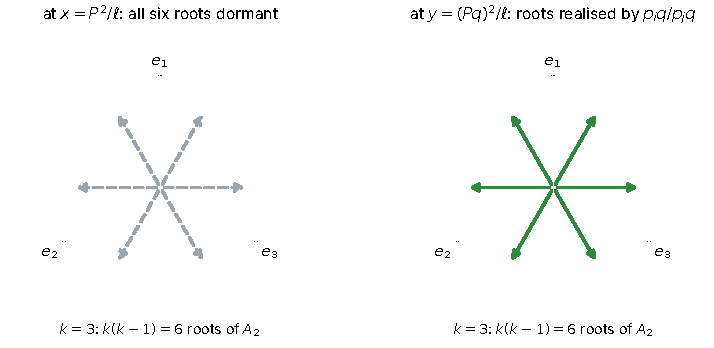
\includegraphics[width=\textwidth]{fig05_dormant_family}
\caption{\textbf{Dormant at $x$, active at $y$ (exact; proved by \cref{thm:A4T1}).} $k=2,3,4$, parameters as in the theorem. Left: $x=P^2/\ell$, a single vertex with the dormant vectors drawn as dashed arrows; right: $y=(Pq)^2/\ell$, the same vectors realised as edges of $K_{k+1}$. The move complex of $y$ is $K_{k+1}$ with no $2$-cells (\cref{thm:A4T2}), so $\beta_1=1,3,6$. The abstract objects are the relations; the geometric object is the cell complex.}\label{fig:dormant}
\end{figure}
\begin{example}[smallest member]\label{ex:A4T1}
$k=2$, $\ell=3$, $c=2$ (order $2$), $p=(5,11)$, $q=2$ ($c^{-1}=2$): $x=55^2/3$, $y=110^2/3$ with $D(y)=\{55,10,22\}$ and $\Kmove(y)$ a triangle. Further instances, $k=2$ with $q=17$ and $k=3,4,5$ with $\ell=7,5,11$, $q=11,3,3$, give $\beta_1=1,3,6,10$; they are recomputed in Appendix~\ref{app:trajectories}. The orbit of $3025/3=55^2/3$ reaches $y$-type structure (with $q=2$, not $17$) after eight steps, \cref{sec:activation}.
\end{example}

\subsection{Persistence of activity; non-persistence of primitivity}
\begin{proposition}[activity is monotone]\label{prop:A4T4a}
Along an orbit, $E_g(x_n)\subseteq E_g(x_{n+1})$ for every $g$ (in universal coordinates). Consequently $\{n:g\text{ is active at }x_n\}=[n_g,\infty)$ for an $n_g\in\N\cup\{\infty\}$.
\end{proposition}
\prov{CW-0431}{A4-T4a}{PROVED}{FULL}
\begin{proof}
In universal coordinates the fibre is the set of exponent vectors of the elements of $D(x_n)$, $F(x_n)=\{\mathrm{exp}(d):d\in D(x_n)\}$, independent of the box. A realisation $\{u,u+g\}$ is a pair of elements of $D(x_n)$, and $D(x_n)\subseteq D(x_{n+1})$ by \cref{lem:M}. \qedhere
\end{proof}
\begin{proposition}[primitivity is not persistent]\label{prop:A4T4b}
Membership $g\in\Gr(x_n)$, the $1$-cells of $\Kmove$ and $\beta_1(\Kmove)$ are not monotone along orbits. Witnesses (\stat{finite-exact}): (i) the vector $e_5-e_{11}$ lies in the lattice of the orbit of $3025/3$ at steps $n=0$ and $n=8$ only, so it is primitive-and-in-$\Gr$ at both ends and absent in between; (ii) at $57$ of the $474$ activation events of the census of \cref{sec:activation} the first Betti number of the move complex drops; (iii) for integers all geometric content is a function of $\sigma$ (\cref{thm:B2T1}), so a new occurrence can enlarge a box and destroy an edge by a divisibility relation.
\end{proposition}
\prov{CW-0432}{A4-T4b}{COUNTEREXAMPLE}{FULL}
\begin{proof}
(i) and (ii) are finite-exact computations (Appendix~\ref{app:trajectories}): along the eight-step orbit the vector $e_5-e_{11}$ is a member of $\Lambda_b\cap[-q,q]$ at $n=0$ and at $n=8$ (both with $b=3$) and of the lattice at none of the states $n=1,\dots,7$, so it is in $\Gr$ at both ends and absent in between. (iii) The orbit of $176^2/7$ at the step $5\to6$ (\cref{ex:zigzag}) has $D=\{8,22,176\}\to D'$ with nine vertices and all three old edges removed. The lattice is the same, but each old edge acquires an intermediate occurrence in its divisor interval (\cref{thm:A5T31}). \qedhere
\end{proof}
